\documentclass[8pt]{beamer}
\usefonttheme[onlymath]{serif}
\newcommand\bmale{\fontsize{6}{7.2}\selectfont}
\newcommand\male{\fontsize{8}{7.2}\selectfont}
\newcommand\normalne{\fontsize{10}{7.2}\selectfont}
\newcommand\duze{\fontsize{12}{7.2}\selectfont}
\setbeamertemplate{caption}{\raggedright\insertcaption\par}

\graphicspath{{commons/}}

 \AtBeginSection[]{
   \begin{frame}
   \vfill
 \centering
   \begin{beamercolorbox}[sep=8pt,center,shadow=true,rounded=true]{title}
     \usebeamerfont{title}\insertsectionhead\par%
   \end{beamercolorbox}
   \vfill
   \end{frame}
 }

\mode<presentation>
{
  \usetheme{CambridgeUS}
  \usecolortheme{beaver}
}
\usepackage{tikz}
\usetikzlibrary{shapes,arrows,positioning}
\tikzstyle{block} = [rectangle, draw, fill=blue!20, rounded corners, align = center, minimum height=2.5cm, minimum width=4cm]
\tikzstyle{line} = [draw, thin, ->, >=stealth]
\tikzstyle{cloud} = [draw, ellipse,fill=red!20, node distance=3cm,    minimum height=2em]

\usepackage{pgfplots}
\usepackage{ulem}
\usepackage{tabto}
\usepackage[]{algorithm2e}
\usepackage{bm}
\usepackage{lmodern}
\usepackage[T1]{fontenc}
\usepackage[polish]{babel}
\usepackage[utf8]{inputenc}
\usepackage{pgfplots}
\usepackage{textcomp}

\DeclareMathOperator*{\argmin}{argmin}
\DeclareMathOperator*{\argmax}{argmax}
\selectlanguage{polish}

\title[Kraków, 2018] % (optional, use only with long paper titles)
{Introduction to Transportation Planning}

\subtitle
{Demand Model, Four Step Demand Model}

\author[dr in\.z. Rafa\l{} Kucharski] % (optional, use only with lots of authors)
{dr in\.z. Rafa\l{} Kucharski\inst{1}}

\institute[] % (optional, but mostly needed)
{
  \inst{1}%
  Katedra System\'{o}w Transportowych\\
  Politechnika Krakowska
 }


\date[KST, L-2, WIL, PK] % (optional, should be abbreviation of conference name)
{Krak\'{o}w, 2018}

\pgfdeclareimage[height=1cm]{university-logo}{commons/ZSK}
 \logo{\pgfuseimage{university-logo}}

\AtBeginSubsection[]
%{
%  \begin{frame}<beamer>{Outline}
%    \tableofcontents[currentsection,currentsubsection]
%  \end{frame}
%}
%\beamerdefaultoverlayspecification{<+->}


\begin{document}

\begin{frame}
  \titlepage
\end{frame}

\section{Demand Model}
\begin{frame}{Demand Model}{}
	\begin{block}{Demand}
		Number of trips $q$ that travellers \alert{demand} to make between origin $o$ and destination $d$.
		\begin{equation}
		q_{od}
		\end{equation}
	\end{block}
	
	\begin{block}{Demand model}
		Estimate the demand
		\begin{equation}
		q_{od} = f(o,d,X_o,X_d,c_{od},\dots)
		\end{equation}
		to determine expected/mean/average demand expressed as a function of known variables $X_o$ and parameters $\bm{\beta}$ estimated to match the observed demand.
	\end{block}
\end{frame}

\section{Travel survey}
\begin{frame}{Travel survey}{Demand model input}
	\begin{block}{Personal Travel diary}
		Chain of trips executed by an individual during the day
	\end{block}
	
	\begin{enumerate}
	\item activity 1: type, location, start time
	\item trip 1: type, location, start time, mode, route
	\item activity 2: type, location, start time
	\item trip 2: type, location, start time, mode, route
	\item activity 3: type, location, start time
	\end{enumerate}
\end{frame}

\begin{frame}{Travel survey}{reason}
	\begin{block}{Survey}
		We cannot know diaries of all individuals (cost, time, organization, privacy, ...). \\ 
		We need to sample the population.	
	\end{block}
	
	\begin{block}{Sampling and extrapolation}
		The sample is representative if the key statistics of the population are the same as for the sample.	
	\end{block}	
\end{frame}

\begin{frame}{Travel survey}{sample sizes}
	\begin{block}{Małopolska 2013}
		12 000 individuals	
	\end{block}
	\begin{block}{Kraków 2014}
		18 000 individuals	
	\end{block}
	
	\begin{block}{Warszawa 2016}
		24 000 individuals	
	\end{block}
	
	\begin{block}{Wrocław 2018}
		300 000 individuals	- GSM traces
	\end{block}
	
\end{frame}

\begin{frame}{Travel survey}{methods}
	\begin{block}{Paper}
		fill the form
	\end{block}
	
	\begin{block}{Tablet}
		fill the form online
	\end{block}
	
	\begin{block}{Census}
		officially fill the form
	\end{block}
	
	\begin{block}{App based}
		install the tracing (GPS) App on your cell phone
	\end{block}
	
	\begin{block}{BigData}
		record anonimized traces - GSM, bluetooth, instargam, etc.
	\end{block}
	
\end{frame}

\begin{frame}{Travel survey}{results}
	\begin{block}{Survey results}
		\begin{enumerate}
		\item average number of trips (per purpose, per person group, per zone)
		\item temporal distribution of trips
		\item trip distance profile/ destination choices
		\item mode shares/mode choices
		\item route choices
		\item vehicle occupancy
		\end{enumerate}	
	\end{block}	
\end{frame}

\begin{frame}{Four step demand model}{FSM}
	\begin{block}{Survey results}
		Reproduce (model) the behaviour read (understood) from survey.
		\\
		Model shall be calibrated, i.e. modelled values shall match the observed (emprical ones)
		
	\end{block}	
\end{frame}

\section{Four step demand model}
\begin{frame}{Four step demand model}{Intro}
\begin{itemize}
\item analitical
\item built on and to reproduce the survey
\item interpretable
\item algorithmic 
\item probabilistic (expected demand)
\item trip based (not chains)
\end{itemize}
\end{frame}

\begin{frame}{Four step model}{FSM}
	\begin{block}{Four step demand model}
		\begin{enumerate}
		\item Trip Generation
		\item * Time Choice
		\item Destination Choice
		\item Mode Choice
		\item Path/Route Choice
		\end{enumerate}	
	\end{block}	
\end{frame}


\begin{frame}{Four step model}{FSM}
\begin{table}[]
\begin{tabular}{l|c|c|c|c}
1 & \textbf{do?/how often?} &  zone production /attraction & $q_o$, $q_d$ & \textbf{Trip Generation}\\ \hline 
2 & \textbf{where?} &  od matrix & $q_{od}$ & \textbf{Destination Choice}\\ \hline 
3 & \textbf{how?} &  mode shares  & $p_{od}$ & \textbf{Mode Choice}\\ \hline 
4 & \textbf{which way?} &  network loads & $q_a$ & \textbf{Route/Path Choice}\\ \hline 
\end{tabular}
\end{table}
\end{frame}

\section{Trip Generation}
\begin{frame}{Trip Generation}
presented on the blackboard at the lecture
\end{frame}

\section{Trip Distribution - Gravity}
\begin{frame}{Destination choice}
\begin{block}{Problem}
We know where trips originate (production) and end (attraction) \\
We \alert{do not know} where the originating trips finish
\end{block}
\begin{block}{Choice}
Traveller:
\begin{itemize}
 \item located in a given place (origin) $o$
 \item has travel demand to be supplied at some destination  
 \item selects (chooses) a place where he supplies his demand
 \end{itemize} 
 \end{block}
\end{frame}

\begin{frame}{Destination choice}{Example 1}
Four travel assignment zones (1-4) generate total of 1000 trips\\
that may be supplied at two destinations: 5 (closer) and 6 (further).
\begin{center}
\begin{minipage}{0.65\textwidth}
        
\begin{tikzpicture}[darkstyle/.style={circle,draw,fill=gray!40,minimum size=10}]

       \node [darkstyle]  (1) at (4,1) {3}; 
       \node [darkstyle]  (2) at (6,3) {2};
       \node [darkstyle]  (3) at (4,3) {1};
       \node [darkstyle]  (4) at (6,1) {4};
       \node [style={rectangle,draw,fill=gray!10,minimum size=20}]  (5) at (5,2) {5};
       \node [style={rectangle,draw,fill=gray!10,minimum size=20}]   (6) at (0,2) {6};
\end{tikzpicture}
    \end{minipage}\hfill
    \begin{minipage}{0.25\textwidth}
     \begin{center}
\begin{tabular}{|c|c|c|}
\hline 
{$o,d$} & P & A \\ 
\hline 
1 & 100 & -  \\ 
\hline 
2 & 200 & -  \\ 
\hline 
3 & 300 & -  \\ 
\hline 
4 & 400 & -    \\ 
\hline 
5 & - & 200  \\ 
\hline 
6 & - & 800  \\ 
\hline
\end{tabular}
\end{center}   
    \end{minipage}
\end{center}

\end{frame}

\begin{frame}{Destination choice}{Example 1}
\begin{center}
\begin{minipage}{0.65\textwidth}
        
\begin{tikzpicture}[darkstyle/.style={circle,draw,fill=gray!40,minimum size=10}]

       \node [darkstyle]  (1) at (4,1) {3}; 
       \node [darkstyle]  (2) at (6,3) {2};
       \node [darkstyle]  (3) at (4,3) {1};
       \node [darkstyle]  (4) at (6,1) {4};
       \node [style={rectangle,draw,fill=gray!10,minimum size=20}]  (5) at (5,2) {5};
       \node [style={rectangle,draw,fill=gray!10,minimum size=20}]   (6) at (0,2) {6};
\end{tikzpicture}
    \end{minipage}\hfill
    \begin{minipage}{0.25\textwidth}
     \begin{center}
\begin{tabular}{|c|c|c|}
\hline 
{$o,d$} & P & A \\ 
\hline 
1 & 100 & -  \\ 
\hline 
2 & 200 & -  \\ 
\hline 
3 & 300 & -  \\ 
\hline 
4 & 400 & -    \\ 
\hline 
5 & - & 200  \\ 
\hline 
6 & - & 800  \\ 
\hline
\end{tabular}
\end{center}   
    \end{minipage}
\end{center}
\begin{block}{Non systematic (non-obligatory) trips with high trip cost impedance} 
e.g. shopping to the closest supermarket (Biedronka)
\end{block}
\begin{center}
\begin{tabular}{|c|c|c|}
\hline 
{$o,d,$}& 5 & 6 \\ 
\hline 
1 & 90 & 10  \\ 
\hline 
2 & 200 & 0 \\ 
\hline 
3 & 270 & 30 \\ 
\hline 
4 & 400 & 0 \\ 
\hline 
\end{tabular} 
\end{center}
\end{frame}

\begin{frame}{Destination choice}{Example 2}
\begin{center}
\begin{minipage}{0.65\textwidth}
        
\begin{tikzpicture}[darkstyle/.style={circle,draw,fill=gray!40,minimum size=10}]

       \node [darkstyle]  (1) at (4,1) {3}; 
       \node [darkstyle]  (2) at (6,3) {2};
       \node [darkstyle]  (3) at (4,3) {1};
       \node [darkstyle]  (4) at (6,1) {4};
       \node [style={rectangle,draw,fill=gray!10,minimum size=20}]  (5) at (5,2) {5};
       \node [style={rectangle,draw,fill=gray!10,minimum size=20}]   (6) at (0,2) {6};
\end{tikzpicture}
    \end{minipage}\hfill
    \begin{minipage}{0.25\textwidth}
     \begin{center}
\begin{tabular}{|c|c|c|}
\hline 
{$o,d$} & P & A \\ 
\hline 
1 & 100 & -  \\ 
\hline 
2 & 200 & -  \\ 
\hline 
3 & 300 & -  \\ 
\hline 
4 & 400 & -    \\ 
\hline 
5 & - & 200  \\ 
\hline 
6 & - & 800  \\ 
\hline
\end{tabular}
\end{center}   
    \end{minipage}
\end{center}
\begin{block}{Non systematic (non-obligatory) trips with highly varying attractivenses} 
e.g. to a restaurant of various attractiveness (reflected in attraction)
\end{block}
\begin{center}
\begin{tabular}{|c|c|c|}
\hline 
{$o,d,$}& 5 & 6 \\ 
\hline 
1 & 20 & 80  \\ 
\hline 
2 & 40 & 160 \\ 
\hline 
3 & 60 & 240 \\ 
\hline 
4 & 80 & 320 \\ 
\hline 
\end{tabular} 
\end{center}
\end{frame}




\begin{frame}{Destination choice}{Example 3}
\begin{center}
\begin{minipage}{0.65\textwidth}
        
\begin{tikzpicture}[darkstyle/.style={circle,draw,fill=gray!40,minimum size=10}]

       \node [darkstyle]  (1) at (4,1) {3}; 
       \node [darkstyle]  (2) at (6,3) {2};
       \node [darkstyle]  (3) at (4,3) {1};
       \node [darkstyle]  (4) at (6,1) {4};
       \node [style={rectangle,draw,fill=gray!10,minimum size=20}]  (5) at (5,2) {5};
       \node [style={rectangle,draw,fill=gray!10,minimum size=20}]   (6) at (0,2) {6};
\end{tikzpicture}
    \end{minipage}\hfill
    \begin{minipage}{0.25\textwidth}
     \begin{center}
\begin{tabular}{|c|c|c|}
\hline 
{$o,d$} & P & A \\ 
\hline 
1 & 100 & -  \\ 
\hline 
2 & 200 & -  \\ 
\hline 
3 & 300 & -  \\ 
\hline 
4 & 400 & -    \\ 
\hline 
5 & - & 200  \\ 
\hline 
6 & - & 800  \\ 
\hline
\end{tabular}
\end{center}   
    \end{minipage}
\end{center}
\begin{block}{Systematic (obligatory) trips with limited attraction capacity} 
e.g. Home-Work with a fixed number of work-places at destination
\end{block}
\begin{center}
\begin{tabular}{|c|c|c|}
\hline 
{$o,d,$}& 5 & 6 \\ 
\hline 
1 & 20 & 80  \\ 
\hline 
2 & 40 & 160 \\ 
\hline 
3 & 60 & 240 \\ 
\hline 
4 & 80 & 320 \\ 
\hline 
\end{tabular} 
\end{center}
\end{frame}

\begin{frame}{Destination choice}{Example 3}
\begin{center}
\begin{minipage}{0.65\textwidth}
        
\begin{tikzpicture}[darkstyle/.style={circle,draw,fill=gray!40,minimum size=10}]

       \node [darkstyle]  (1) at (4,1) {3}; 
       \node [darkstyle]  (2) at (6,3) {2};
       \node [darkstyle]  (3) at (4,3) {1};
       \node [darkstyle]  (4) at (6,1) {4};
       \node [style={rectangle,draw,fill=gray!10,minimum size=20}]  (5) at (5,2) {5};
       \node [style={rectangle,draw,fill=gray!10,minimum size=20}]   (6) at (0,2) {6};
\end{tikzpicture}
    \end{minipage}\hfill
    \begin{minipage}{0.35\textwidth}
     \begin{center}
\begin{tabular}{|c|c|c|}
\hline 
{$o,d$} & P & A \\ 
\hline 
1 & 100 & -  \\ 
\hline 
2 & 200 & -  \\ 
\hline 
3 & 300 & -  \\ 
\hline 
4 & 400 & -    \\ 
\hline 
5 & - & 200 \alert{-> 800}  \\ 
\hline 
6 & - & 800 \alert{-> 200} \\ 
\hline
\end{tabular}
\end{center}   
    \end{minipage}
\end{center}
\begin{block}{Systematic (obligatory) trips where supply eventually matched the demand} 
e.g. preschool locations moving closer to children
\end{block}
\begin{center}
\begin{tabular}{|c|c|c|}
\hline 
{$o,d,$}& 5 & 6 \\ 
\hline 
1 & 80 & 20  \\ 
\hline 
2 & 1600 & 40 \\ 
\hline 
3 & 240 & 60 \\ 
\hline 
4 & 320 & 80 \\ 
\hline 
\end{tabular} 
\end{center}
\end{frame}

\begin{frame}{Actual trip distribtuion structure}{Reflected in the GSM traces}
\begin{figure}
\begin{center}
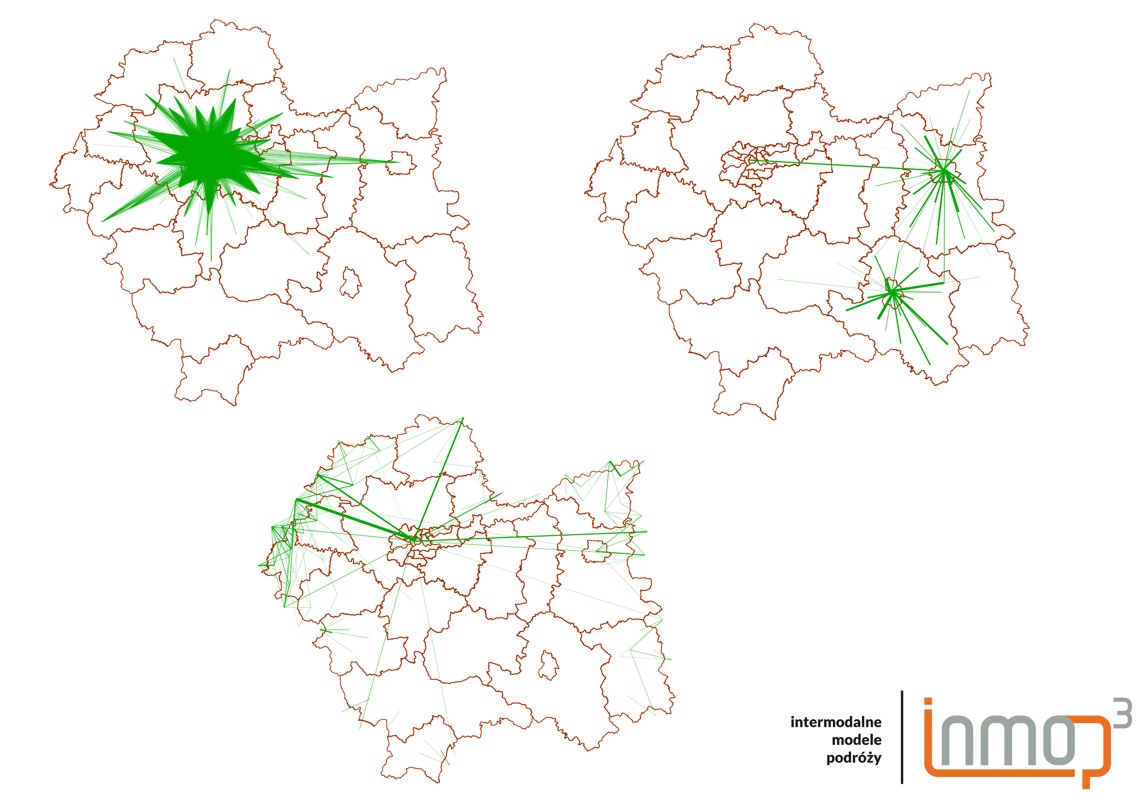
\includegraphics[height=7cm]{8}
 \end{center}
 \end{figure} 
 \end{frame}
 
\begin{frame}{Gravity model}{Formalization}
\begin{block}{Proportional model}
If we assume that the only factor in trip choices is attractivity, we get:
\begin{equation*}
Q_{od}=f(P_o,A_d) = \frac{P_o}{\sum_{o \in Z} P} A_d = P_o \frac{A_d}{\sum_{d \in Z} A}
\end{equation*}
\\
we may read it as:\\
1. distribute production proportionally to attraction
\begin{equation*}
Q_{od}=P_o \frac{A_d}{\sum_{d \in Z} A}
\end{equation*}
2. distribute attraction proportionally to production
\begin{equation*}
Q_{od}=A_d \frac{P_o}{\sum_{o \in Z} P}
\end{equation*}
\end{block}
one of production/attraction needs to be in absolute values (trips) second one may be just proportionality factor
\end{frame}

\begin{frame}{Gravity model}{Formalization}
Problem with proportional model: \alert{no distance included}
\begin{block}{Gravity model}
If in proportional model we include distance function (cost $c_od$), we get:
\begin{equation*}
Q_{od}=f(P_o,A_d, c_{od}) = f(c_od) \frac{P_o}{\sum_{o \in Z} P} A_d 
\end{equation*}
\end{block}
\end{frame}

with two specific functions to apply:

\begin{frame}{Gravity model}{Cost functions}
\begin{tikzpicture}[declare function={
f(\x,\y)=(\y/\x)* (1/sqrt(2*pi*1))*exp(-(ln(\x/\y)-0)^2/(2*1);
{]
      \draw[->] (0,0) -- (16,0) node[right] {$x$};
      \draw[->] (0,0) -- (0,4) node[above] {$y$};
      \draw[scale=0.5,domain=0:16,smooth,variable=\x,blue] plot ({\x},{10*exp(-\x*0.2)});
      \draw[color=green!60!black,very thick,domain=0.01:200,samples=101]{f(x,100)};
          \end{tikzpicture}
\end{frame}

\begin{frame}{Summary}{Thanks for attention}
Rafal Kucharski, rkucharski(at)pk.edu.pl
\end{frame}

\end{document}



